\documentclass[12pt]{report}
\usepackage{thesis}
\usepackage[pdftex]{graphicx}
\usepackage[utf8]{inputenc}
\usepackage{amsmath}

\title{LEARNING LIKE A HUMAN IN COGNITIVE ROBOTS \\ METHODOLOGY REPORT}

\author{Semih Onay}

\program{Computer Science}

\supervisor{Assistant Professor Elena Battini Sönmez}

\begin{document}

\makecstitle

\chapter{INTRODUCTION}

\pagenumbering{arabic}

The iCub is a humanoid robot developed at Istituto Italiano di Tecnologia (IIT) as part of the European project RobotCub and later adopted by more than 20 laboratories worldwide.It has 53 motors that move the head, arms \& hands, midriff, and legs.It can see and hear, it has the sense of proprioception (body configuration) and movement (using accelerometers and gyroscopes).It's designed to aid studies of human cognition and artificial intelligence.Project members have developed computer simulator for experimenting new techniques.\cite{iCub}

Computer simulations are getting important in area robotics area.Simulations may not provide real complexity of physical world and not reliable as real one.A simulator for the iCub is an easy way to test new algorithms and methods instead of dealing with complex configuration of iCub robot.
\begin{figure}[!h]
\begin{center}
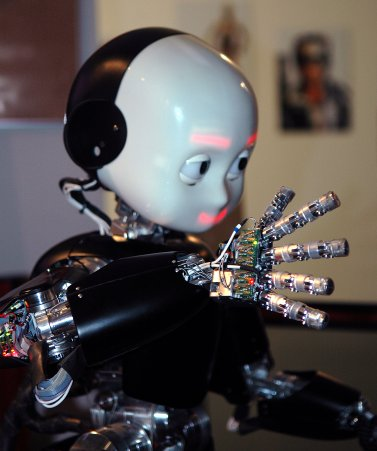
\includegraphics[scale=1.7]{iCub.jpg}
\caption{iCub}
\end{center}
\end{figure}
The iCub simulator is designed to be as accurate as real world psychics and dynamics.Construction based on directly from first prototype simulation environment Webots\cite{webots}.Webots is expensive and had limited access to source code which made hard to modify source code in order to add some properties.Then iCub simulation created.Simulation environment uses ODE(Open Dynamics Engine)\cite{ode} to simulate body movement and collision detection algorithms to measure psychical interaction with the world.ODE is used in wide range of projects like Gazebo project.\cite{gazebo}ODE is an open source physics engine for authoring tools, computer games,etc.It uses OpenGL renderer and it has some disadvantages due to limitation of OpenGL engine computation efficiency on complex structures.iCub simulation uses OpenGL directly via SDL which helps to render complex robot movements and computation efficient simulation observations.\cite{sdl} Simulator is free and available to anyone who interested in robotics and learning about basics of robotics.
\newpage
\chapter{Methodology}

Research will go on a computer simulation model of the iCub robot.The simulator allows to create realistic scenarios in where robot can interact with a virtual world and physical limitations and interactions that occur between the virtual world is simulated using open source library which is ODE (Open Dynamics Engine) to provide accurate simulation of body dynamics.
\begin{figure}[!h]
\begin{center}
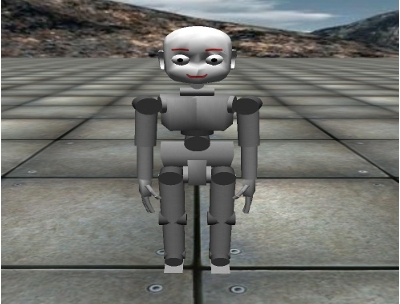
\includegraphics[scale=1.3]{iCubSim.jpg}
\caption{iCub on simulation}
\end{center}
\end{figure}
The iCub simulation was developed on the top of YARP(Yet Another Robot Platform)\cite{yarp}.YARP is a set of open source libraries that supports modularity by using abstraction method in softwares to handle common difficulties in robotics area which are know as modularity algorithms and hardware interfaces and OS platforms.To deal with OS spesific builds,requires to use cross-platform build tools such as CMake\cite{cmake} and ACE\cite{ace}.

YARP is providing platform independence.First abstraction can be described as a protocols.Main YARP protocol manages inter-process communications in operating systems.It can deliver process messages of any size across the network by using different protocols.
\newpage
Second abstraction is about hardware communications.The method is to define interface for class of devices to fold native coded APIs.Changes in hardwares requires changes in API calls via linking suitable libraries to encapsulate hardware dependency problems.
These two abstraction combined to use remote device drives where that can be accessed across the network like a parallel processing.

\begin{figure}[!h]
\begin{center}
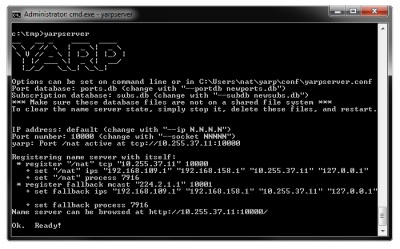
\includegraphics[scale=1.0]{yarpServer.jpg}
\caption{yarpServer running on Windows x86}
\end{center}
\end{figure}

\begin{figure}[!h]
\begin{center}
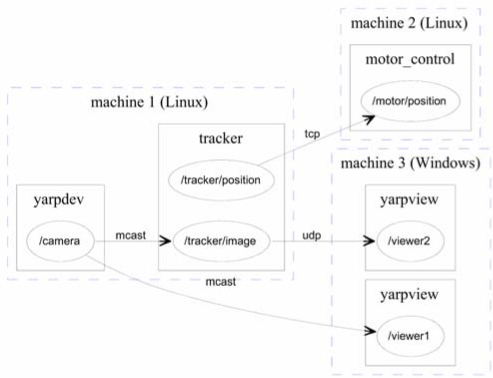
\includegraphics[scale=0.4]{network.jpg}
\caption{YARP Work Flow}
\end{center}
\end{figure}
The purpose of YARP ports are to move data from threads to threads over the processes.Flow of the data can be configured and observed from command-line at real-time.Port can receive or send data from any other port.Connections between ports can be modified easily with using different protocols such as TCP(Transmission Control Protocol) and UDP(User Datagram Protocol).The choice of protocol is depends on quality of message transmission or response time.Using TCP is for reliability and UDP is for speed with effect on unreliable transmissions.


\begin{thebibliography}{9}
\bibitem{iCub}iCub : icub.org
\bibitem{webots}Webots : cyberbotics.com
\bibitem{ode}ODE(Open Dynamics Engine) : opende.sourceforge.net
\bibitem{gazebo}GAZEBO : gazebosim.org
\bibitem{sdl}SDL : libsdl.org
\bibitem{figure}Figure 1.1 : "iCub science festival" by Lorenzo Natale
\bibitem{cmake}CMake : cmake.org 
\bibitem{ace}Adaptive Communication Environment : dre.vanderbilt.edu/~schmidt/ACE.html
\bibitem{resource}The iCub humanoid robot:an open platform for research in embodied cognition,Giorgio Metta,Giulio Sandini,David Vernon,Lorenzo Natale,Francesco Nori
\bibitem{resource}The iCub Humanoid Robot Simulator,V.Tikhanoff, P.Fitzpatrick, F.Nori, L Natale, G.Metta and A.Cangelosi
\bibitem{resource}An Open-Source Simulator for Cognitive Robotics Research: The Prototype of the iCub Humanoid Robot Simulator,V.Tikhanoff, P.Fitzpatrick, F.Nori, L Natale, G.Metta and A.Cangelosi
\end{thebibliography}
\newpage
\end{document}
